% !TEX TS-program = XeLaTeX
% use the following command:
% all document files must be coded in UTF-8
\documentclass[english]{textolivre}
% build HTML with: make4ht -e build.lua -c textolivre.cfg -x -u article "fn-in,svg,pic-align"

\journalname{Texto Livre}
\thevolume{16}
%\thenumber{1} % old template
\theyear{2023}
\receiveddate{\DTMdisplaydate{2023}{3}{11}{-1}} % YYYY MM DD
\accepteddate{\DTMdisplaydate{2023}{4}{12}{-1}}
\publisheddate{\DTMdisplaydate{2023}{7}{5}{-1}}
\corrauthor{Elaine Cristina Gomes Aires de Oliveira}
\articledoi{10.1590/1983-3652.2023.45190}
%\articleid{NNNN} % if the article ID is not the last 5 numbers of its DOI, provide it using \articleid{} commmand 
% list of available sesscions in the journal: articles, dossier, reports, essays, reviews, interviews, editorial
\articlesessionname{articles}
\runningauthor{Oliveira and Lima} 
%\editorname{Leonardo Araújo} % old template
\sectioneditorname{Daniervelin Pereira}
\layouteditorname{Thaís Coutinho}

\title{Instagram, fast food and Historical-Critical Pedagogy: ingredients for the discourse in favor of healthy eating in the context of teaching English}
\othertitle{Instagram, \textit{fast food} e Pedagogia Histórico-Crítica: ingredientes para o discurso a favor de uma alimentação saudável no contexto de ensino de inglês}
% if there is a third language title, add here:
%\othertitle{Artikelvorlage zur Einreichung beim Texto Livre Journal}

\author[1]{Elaine Cristina Gomes Aires de Oliveira~\orcid{0000-0002-1022-4687}\thanks{Email: \href{mailto:elaine.cristina.aires@gmail.com}{elaine.cristina.aires@gmail.com}}}
\author[2]{Samuel de Carvalho Lima~\orcid{0000-0002-7145-3686 }\thanks{Email: \href{mailto:samuel.lima@ifrn.edu.br}{samuel.lima@ifrn.edu.br}}}
\affil[1]{Centro Estadual de Educação Profissional Professor Francisco de Assis Pedrosa, Mossoró, RN, Brasil.}
\affil[2]{Instituto Federal de Educação, Ciência e Tecnologia do Rio Grande do Norte, Mossoró, RN, Brasil.}

\addbibresource{article.bib}
% use biber instead of bibtex
% $ biber article

% used to create dummy text for the template file
\definecolor{dark-gray}{gray}{0.35} % color used to display dummy texts
\usepackage{lipsum}
\SetLipsumParListSurrounders{\colorlet{oldcolor}{.}\color{dark-gray}}{\color{oldcolor}}

% used here only to provide the XeLaTeX and BibTeX logos
\usepackage{hologo}

% if you use multirows in a table, include the multirow package
\usepackage{multirow}

% provides sidewaysfigure environment
\usepackage{rotating}

% CUSTOM EPIGRAPH - BEGIN 
%%% https://tex.stackexchange.com/questions/193178/specific-epigraph-style
\usepackage{epigraph}
\renewcommand\textflush{flushright}
\makeatletter
\newlength\epitextskip
\pretocmd{\@epitext}{\em}{}{}
\apptocmd{\@epitext}{\em}{}{}
\patchcmd{\epigraph}{\@epitext{#1}\\}{\@epitext{#1}\\[\epitextskip]}{}{}
\makeatother
\setlength\epigraphrule{0pt}
\setlength\epitextskip{0.5ex}
\setlength\epigraphwidth{.7\textwidth}
% CUSTOM EPIGRAPH - END

% LANGUAGE - BEGIN
% ARABIC
% for languages that use special fonts, you must provide the typeface that will be used
% \setotherlanguage{arabic}
% \newfontfamily\arabicfont[Script=Arabic]{Amiri}
% \newfontfamily\arabicfontsf[Script=Arabic]{Amiri}
% \newfontfamily\arabicfonttt[Script=Arabic]{Amiri}
%
% in the article, to add arabic text use: \textlang{arabic}{ ... }
%
% RUSSIAN
% for russian text we also need to define fonts with support for Cyrillic script
% \usepackage{fontspec}
% \setotherlanguage{russian}
% \newfontfamily\cyrillicfont{Times New Roman}
% \newfontfamily\cyrillicfontsf{Times New Roman}[Script=Cyrillic]
% \newfontfamily\cyrillicfonttt{Times New Roman}[Script=Cyrillic]
%
% in the text use \begin{russian} ... \end{russian}
% LANGUAGE - END

% EMOJIS - BEGIN
% to use emoticons in your manuscript
% https://stackoverflow.com/questions/190145/how-to-insert-emoticons-in-latex/57076064
% using font Symbola, which has full support
% the font may be downloaded at:
% https://dn-works.com/ufas/
% add to preamble:
% \newfontfamily\Symbola{Symbola}
% in the text use:
% {\Symbola }
% EMOJIS - END

% LABEL REFERENCE TO DESCRIPTIVE LIST - BEGIN
% reference itens in a descriptive list using their labels instead of numbers
% insert the code below in the preambule:
%\makeatletter
%\let\orgdescriptionlabel\descriptionlabel
%\renewcommand*{\descriptionlabel}[1]{%
%  \let\orglabel\label
%  \let\label\@gobble
%  \phantomsection
%  \edef\@currentlabel{#1\unskip}%
%  \let\label\orglabel
%  \orgdescriptionlabel{#1}%
%}
%\makeatother
%
% in your document, use as illustraded here:
%\begin{description}
%  \item[first\label{itm1}] this is only an example;
%  % ...  add more items
%\end{description}
% LABEL REFERENCE TO DESCRIPTIVE LIST - END


% add line numbers for submission
%\usepackage{lineno}
%\linenumbers

\begin{document}
\maketitle

\begin{polyabstract}
 
\begin{english}
\begin{abstract}
The purpose of this article is to analyze the discourse of high school students in favor of healthy eating in the context of English language teaching in a public professional education school. Based on Dialogic Discourse Analysis, a \emph{corpus} composed of 2 posts on Instagram by high school students enrolled in the technical course of Nutrition and Dietetics who produced verbal-visual texts during an action research with English classes inspired by Historical-Critical Pedagogy is explored. The analysis of the posts reveals that the discourse in favor of healthy eating is interrelated with the technical discourse, the everyday discourse, and the discourse about the consequences of fast food consumption. The analysis also shows that the posts have a negative value emphasis in relation to the consumption of fast food, and, through the pamphlet and the informative poster, they denounce the dangers of unhealthy food choices, also seeking to raise awareness among their interlocutors and promote a change in the social practice of these subjects. It is concluded that English classes inspired by Historical-Critical Pedagogy provide students with opportunities to disseminate discourses in a far-reaching social network, expanding their interlocutors, committing themselves to collaborate for a society that is more aware of its eating habits.

\keywords{English language teaching \sep Historical-Critical Pedagogy \sep Dialogic discourse analysis \sep Public school \sep Professional education}
\end{abstract}
\end{english}

\begin{portuguese}
\begin{abstract}
O objetivo deste artigo é analisar o discurso de estudantes de ensino médio a favor de uma alimentação saudável no contexto de ensino de língua inglesa em uma escola pública de educação profissional. A partir da Análise Dialógica do Discurso, explora-se um \emph{corpus} composto por duas postagens no Instagram de estudantes do ensino médio integrado ao curso técnico de Nutrição e Dietética que produziram textos verbo-visuais durante uma pesquisa-ação com aulas de inglês inspiradas na Pedagogia Histórico-Crítica. A análise das postagens revela que o discurso a favor de uma alimentação saudável se inter-relaciona com o discurso técnico, o discurso do cotidiano e o discurso sobre as consequências do consumo de \emph{fast food}. A análise também evidencia que as postagens apresentam uma ênfase valorativa negativa em relação ao consumo de \emph{fast food}, e, por meio do panfleto e do cartaz informativo, denunciam os perigos de escolhas alimentares não saudáveis, buscando, ainda, conscientizar seus interlocutores e promover uma mudança na prática social desses sujeitos. Conclui-se que as aulas de inglês inspiradas na Pedagogia Histórico-Crítica oportunizam aos estudantes circular discursos em uma rede social de grande alcance, ampliando seus interlocutores, comprometendo-se a colaborar para uma sociedade mais consciente dos seus hábitos alimentares.

\keywords{Ensino de língua inglesa \sep Pedagogia Histórico-Crítica \sep Análise dialógica do discurso \sep Escola pública \sep Educação profissional}
\end{abstract}
\end{portuguese}
% if there is another abstract, insert it here using the same scheme
\end{polyabstract}

\section{Introduction}

The National Common Curricular Base (BNCC) for High School guides that learning English should allow students to use the language to deepen their understanding of the world they live in, expanding their discursive capacity and reflection in different areas of knowledge \cite{brasilministeriocurricular}. In response to this regulation, public school students need the necessary conditions to become critical subjects in the society in which they participate, using the English language as a lingua franca. Based on this premise, in the field of Applied Linguistics (AL), teacher-researchers have created intelligibility about English language teaching committed to the students’ most immediate reality, considering the social problems they are aware of \cite[among others]{urzeda-freitas_educando_2012, costados2011visualizaccao, mulico_learning_2020, lima_ensino_2021, limade2020whatsapp}.

Aligning with the AL that seeks to create intelligibility about social problems in which language plays a central role \cite{moita2006linguistica}, this article assumes the interdisciplinary nature of this field of study and adopts 2 theoretical perspectives to problematize the teaching of the English language in public school, that is, a theory of language and a pedagogical theory, respectively, Dialogic Discourse Analysis (DDA) and Historical-Critical Pedagogy (HCP). In this way, the teaching of the English language is discussed from the DDA, assuming that the discourse is always fused in the form of an utterance belonging to a certain individual, and outside of this form it cannot exist, assuming that one learns to use the language in the discursive exchange, in the use of language, when interacting with other people via language \cite{bakhtin_os_2016}.

Given this, this article aims to analyze the discourse of high school students in favor of healthy eating in the context of English language teaching in a public school of professional education. Based on the DDA, a \emph{corpus} composed of 2 posts on Instagram - an online social network for sharing photos and videos - by high school students enrolled in the technical course of Nutrition and Dietetics who produced verbal-visual texts during an action research with English classes inspired by HCP is explored. Therefore, by mobilizing Instagram as a social network for the dissemination of texts after debating the topic of fast food consumption in English classes inspired by the HCP, it is possible to gather the necessary ingredients for the production of the discourse in favor of a healthy diet, as pointed out in the title of the article, although this study does not intend to prescribe an intransigent culinary recipe.

To shape this discussion, the article is organized into 6 sections. In addition to this introduction, the next section presents the research affiliation to the DDA. Subsequently, the teaching of English inspired by HCP is described. For the data analysis, the discourse of high school students in favor of healthy eating is explored in sections results and discussion. Finally, in the final considerations, the pedagogical and methodological implications of the investigation are presented.


\section{Dialogic Discourse Analysis}

According to \textcite{brait_bakhtin_2020}, Dialogic Discourse Analysis (DDA) can be understood as approaching a discursive corpus from the concepts developed in the set of works produced from the beginning of the 20th century, in Russia, by a multidisciplinary group of intellectuals who became known for Bakhtin and the Circle (Bakhtin, Volóchinov, Medvedev, among others). This group explored different topics, among them the language, topic of interest of this investigation. Thus, Bakhtin and the Circle have deserved, in recent years, great attention from different areas of knowledge, a fact that can be “verified in the countless translations, in the countless interpretative essays and, especially, in the dissemination of notions, categories, concepts arising directly from Bakhtinian thought, presented with him or even motivated by him”\footnote{Original: “constatado nas inúmeras traduções, nos incontáveis ensaios interpretativos e, especialmente, na circulação de noções, categorias, conceitos advindos diretamente do pensamento bakhtiniano, com ele aparentados ou ainda, por ele motivados”.} \cite[p. 8]{brait_bakhtin_2020}.

In DDA, language is understood as a discursive interaction and, from there, the utterance is the real unit of the discursive flow, formed between 2 socially organized individuals, situated in a determined time and space, therefore culturally established, so that, in the absence of a real interlocutor, the image of the average representative of that social group is considered \cite{volochinov2018}. In other words, every utterance responds to something and is oriented towards a presumed answer and, therefore, participates in what Volóchinov understands as a large-scale ideological discussion, since every utterance responds, refutes, confirms, complements other utterances, which guarantees its dialogic nature.

Thus, for \textcite[p. 71-80]{bakthin1986}, “The utterance is not a conventional unit, but a real unit, clearly delimited by the change of speaking subjects, which ends by relinquishing the floor to the other, as if with a silent \emph{dixi}, perceived by the listeners (as a sign) that the speaker has finished”\footnote{For direct quotes, Bakhtin’s work translated into English was used: BAKHTIN. Mikahil. Speech Genres and Other Late Essays. Texas - Usa: University Of Texas Press, 1986. Translated by Vern W. McGee.}. Constituting a key concept in Bakhtinian theory, the utterance is understood as a link in the discursive interaction, so that in every utterance “we embrace, understand, and sense the speaker‘s \emph{speech plan or speech will}, which determines the entire utterance, its length and boundaries. \cite[p.77, emphasis in original]{bakthin1986}.

In addition, in this theoretical-methodological perspective, the study of language presumes to consider the fields of human activity, since each field elaborates its speech genres, that is, its relatively stable types of utterances \cite{bakhtin_os_2016}. In the context of English language teaching in a public school, the teacher’s field of professional activity, several utterances are produced in the interaction between teacher and student, and student and student, namely: the explanation of an activity, the request to go to the toilets, numerous replications of conversations between students, among others. In addition, many utterances that are produced and are disseminated in other fields of human activity are explored by the teacher and students to carry out activities of reading and writing texts, namely: journalistic news, advertisements, cooking recipes, song lyrics, among others.

Adopting, in the English language class, utterances that disseminate in different fields of human activity, in a dialogic perspective, is not new. Considering these utterances as verbal-visual texts, and analyzing them later to create intelligibility about language teaching, neither. To cite an example, \textcite{limade2022auto} uses memes in the context of teaching English in a 60-minute remote class for Youth and Adults. When carrying out a DDA of the material used, based on the interpretation that memes are verbal-visual texts, the author finds that the verbal language of memes responds creatively to images of scenes from a Brazilian soap opera and a Hollywood film, promoting the denunciation of the lack of democratization of internet access, a meaning produced in the context of teaching the English language in public schools, and which goes beyond the walls of the school, as this discourse circulated more strongly in the daily life of a society that was going through a pandemic and social isolation in 2020. This discussion points, therefore, to the potentiality of the English language class as a space/time in which there is the emergence of discourses that critically reflect on social problems, which can also be observed in the classes inspired by the HCP, subsequently reported in this article.

To analyze memes that disseminate in social networks, \textcite{limade2022auto} adopted the perspective of verbal-visual utterances, so that, as proposed by \textcite{brait_olhar_2013}, in these texts, both verbal language and visual language play a constitutive role in the production of meanings, not they can be separated, which also applies to the corpus analyzed in this article. In the next section, therefore, the teaching of English inspired by Historical-Critical Pedagogy is described, highlighting the context of the production of the texts that constitute the corpus to be analyzed, that is, posts on Instagram, which are taken as verbal-visual utterances from the DDA.


\section{Teaching English inspired by Historical-Critical Pedagogy}

The critical teaching of English aimed at the development of critical thinking is the context of the production of the corpus of this article. The study recognizes that critical teaching is an object of investigation and reflection in an international context \cite{ahangari2014effect, bobkina_literature_2016, sobkowiak_critical_2016, suarcaya2017investigating, sadeghi2020iranian}. However, the conception adopted is the one that assumes that critical teaching emerges from “research of Brazilian English teachers-researchers who relate the teaching-learning of English to social problems”\footnote{Original: “pesquisas de professores-pesquisadores de inglês brasileiros que relacionam o ensino-aprendizagem de inglês a problemas sociais”.}\cite[p. 141]{lima_ensino_2021} is adopted. Thus, in the field of Brazilian Applied Linguistics (AL), there are already records of what has been conceived as critical teaching of the English language \cite[among others]{urzeda-freitas_educando_2012, costados2011visualizaccao, caetano_but_2020, mulico_learning_2020}. In this wake, this topic is productive, although it needs to be expanded in order to build a body of knowledge that reflects a set of systematic practices to promote criticality in English classes in public schools. Thus, by continuing this production of knowledge, expanding it is intended, in this case, relating the teaching of English to Historical-Critical Pedagogy (HCP).

In the formal teaching context, whoever assumes the role of an educational agent has already been through school in some way, having experienced, therefore, even if unsystematically, educational theories that are materialized in different pedagogical practices. This implies stating that teachers and pedagogues tend to move from one theoretical orientation to another, among those that are in circulation, depending on the circumstances. For \textcite{saviani_pedagogia_2019}, these theories are those that correspond to the dominant ideas, belonging to the ideas of the dominant classes, that is, hegemonic theories, which are presented as corresponding to the interests of the whole society, even though they are not.

According to \textcite[p.18]{galvao2019fundamentos}, in opposition to hegemonic theories, HCP positions itself as a theory aligned with the demands of the working class. In this way, thinking about teaching English inspired by the HCP demands a look at learning that mobilizes the student to perceive the environment in which they live, as well as the possibilities of transforming it in a critical way. Thus, for \textcite{saviani_pedagogia_2019}, it is up to critical theory to position itself in line with the interests of the dominated in order to be able to dismantle hegemonic theories based on social, historical, and epistemological contextualization.

Understanding work as an educational principle, Saviani points out that throughout the formal school journey the relationship between work and education is present. In secondary education, the relationship between education and work, between knowledge and practical activity, should be dealt with explicitly and directly. Knowledge has relative autonomy in relation to the work process from which it originates.

\begin{quote}
 The fundamental role of high school will therefore be to recover this relationship between knowledge and work practice. Thus, in secondary education it is no longer enough to master the basic and general elements of knowledge that result from and at the same time contribute to the work process in society. It is now a question of explaining how knowledge (specific object of the teaching process), that is, how science, spiritual power, becomes material power in the production process. Such explanation must involve not only theoretical, but also practical mastery of how knowledge is articulated with the productive process\footnote{Original: “no ensino médio já não basta dominar os elementos básicos e gerais do conhecimento que resultam e ao mesmo tempo contribuem para o processo de trabalho na sociedade. Trata-se, agora, de explicitar como o conhecimento (objeto específico do processo de ensino), isto é, como a ciência, potência espiritual, se converte em potência material no processo de produção. Tal explicitação deve envolver o domínio não apenas teórico, mas também prático sobre o modo como o saber se articula com o processo produtivo”.}. \cite[p.160]{saviani_trabalho_2007}.
\end{quote}


In this way, society is organized and transformed through work, and this is socially and culturally established through the formal schooling process. In this schooling process, critical teaching of the English language is no longer established in a language decoding process, but rather as a process of dialog between cultures and societies.

The teaching of English inspired by the HCP must provide the student with a horizontal look at the world, seeing the social problems that surround them and seeking mechanisms to solve them. Based on this assumption, in 2022, an action research was done in the English classes of a public professional education school in order to give students the opportunity to reflect on a social problem in evidence today, articulating this problem with the proposal of professional education of the technical course in which the students were enrolled, the Integrated Technical Course of Nutrition and Dietetics. The action research was carried out after approval by the Research Ethics Committee (REC) – number 5.518.567 by Federal Institute of Rio Grande do Norte. The age group of the action research participants was 14 to 17 years old. The issue addressed was the challenge of healthy eating, opposing the consumption of fast food, which was incorporated into the eating habits of the Brazilian population, especially the young public, participants of the action research.

The English language classes took place from September to October 2022 in a third-grade class of the Integrated Technical Course in Nutrition and Dietetics at a public professional education school located in the Oeste Potiguar, where the first author of the article is a teacher. During the classes, the students discussed and reflected on fast food advertisements, noticing a recurrent use of warm and vibrant colors and, when the texts disseminated in a local (Brazilian) context, it was also noticed the insertion of the English language as a way to attribute prestige to the advertised product.

Therefore, action research with English classes inspired by the HCP was carried out by planning 10 classes (1 class = 50 minutes), discussing the consumption of fast food. The classes had a sequence according to the moments recommended by the HCP, namely: \emph{social practice, problematization, instrumentalization, catharsis and social practice} \cite{saviani_pedagogia_2019}.

For social practice, 1 class was held with the presentation of advertisements from local companies that sell fast food. To start this class, the proposal of 10 classes based on the topic of fast food was presented to the class. The students were also shown the need to discuss this topic in a society that has talked a lot about healthy eating and, on the other hand, has eating habits that are harmful to health. After a brief discussion on the topic, images of local commercial establishments linked to fast food were presented. As the images were displayed, an attempt was made to understand the consumption relationships that the students had with this type of food and how they perceived the connection of the English language in the means of advertising the products. During the class students could perceive themselves as consumers, or not, of the products presented.

 For problematization, 2 classes were held in which students analyzed posters of global fast food chains, identifying the verbal-visual characteristics used in advertisements. Similar to the previous class, in this second moment, images of advertisements from companies that have fast food as their main marketing item were presented to the class. However, the focus was no longer on local businesses, but on large national and international fast food chains. Because it was a large class (38 students) and understanding the importance of collaborative work, the class was divided into groups of up to 5 people. The students were instructed to form groups according to their personal affinities, since for a better use of the activity it would be important for the students to be as comfortable as possible. Once the groups were formed, the previously selected images were presented by the data show and the students were asked to write about: \emph{a. The resources found (images, colors, fonts, etc.) to attract the interlocutor to the consumption of those foods; b. How the English language influences the advertising presented; and c. How the use of English in advertisements can influence Brazilian culture}. For each image presented, 5 minutes were given for students to make their notes. After the presentation of all the images, the points presented by the students were discussed.

For instrumentalization, 2 classes were held to watch a video about the history of fast food and to create a timeline on the chronology of the video, and 2 classes were held to read and discuss an abstract of a scientific article selected by the students on the topic \emph{fast food/healthy eating}. Before playing the video for the class, students were asked what they knew about fast food in terms of its origin and how it arrived in Brazil. Those who responded generally said that fast food came from the United States along with the McDonald’s chain and that Brazilians had already appropriated this food culture. Other students pointed out that nowadays, especially in big cities, the habit of eating fast food for lunch has become increasingly common. Students were asked to talk about their notes and impressions about the video they had watched. It was noticeable that the methodology used worked, as all groups were able to verbalize the most important points of the video, which was to realize that the fast food culture, although it seems to be recent, goes back a long time. The discussion about the influence of an American and European culture on Brazilian culture was also brought up at that moment.

Finally, for catharsis and social practice, 3 classes were held to create posts for Instagram, considering that the potential of this social network to involve students in foreign language teaching practices were well-evaluated by previous research \cite{prasetyawati2020integrating, aghayi2021instagram, garcia2022you, andujar2023foreign}. For that, students were questioned about their opinion on creating an Instagram profile to publicize their work and alert people to more assertive food choices. The response obtained was very enthusiastic and interested in participating. Therefore, students were asked to form pairs during the class and prepare a post about what they considered most pertinent to be presented about what they had worked on in previous classes. The focus of the post was not limited precisely to understand which aspects were most relevant from the students’ point of view and how the classes had impacted their view of fast food culture. The only requirement was that the post should be in English and that they create three hashtags so that the post could have a greater reach on the internet, as they would be linked to a chain of posts that used the same hashtag. All students had cell phones with internet access, so they did not need to use other materials. Not all students were able to complete the activity in the classroom, so they needed to finish the task at home.

Among many utterances produced in the flow of communication between research participants, in this article, the corpus selected for analysis consists of 2 posts made by students on the social network Instagram. The posts were created by the students as a proposed activity to contemplate the \emph{catharsis and social practice} foreseen in the HCP, that is, its last moments. We resorted to the moment of \emph{catharsis and social practice} because we understood that, based on the students’ responses to the activities, it would be possible to capture the impacts of the action research on the participants, thus evaluating the teaching of English inspired by the HCP, through the discourse produced and disseminated by them.

Based on the DDA, the 2 posts on Instagram are interpreted as students’ responses to their experiences in English classes, considering the guidelines given by the teacher in relation to how to proceed in preparing their texts: clarity of content, observance of the appropriate use of English, hashtags that had the maximum reach for the topic. In addition, the posts are also interpreted as links in the chain of discursive interaction, that is, establishing relationships with utterances that are produced and circulated in a less immediate context of the students. The teacher-researcher did not delimit the focus of the posts, the only requirement being that it would establish a relationship with the topic of the classes, the consumption of fast food.

Thus, the procedure for analyzing the 2 posts that constitute the corpus of this research took place in a theoretical-methodological perspective of the DDA, that is, as discussed by \textcite{rohling2014pesquisa}, considering the complex relationship (dialogic and constitutive) between the researcher and the research object. Such a relationship is neither neutral nor predetermined, considering that the researcher, throughout the research process, is also permeated by their evaluative horizon, preponderant in their choices during the research process, ranging from the choice of the object to the report of the data analysis.

Finally, in order to explore the posts taken as utterances/texts from the DDA, the methodologically grounded order for the study of the language, as foreseen by \textcite{volochinov2018}, is adopted, performing the analysis of the forms and types of discursive interaction in its relation to concrete conditions, the analysis of the forms of utterances or singular discourses in close relation with the interaction of which they are part, and the analysis of the forms of language in its usual linguistic conception. In the following section, results are presented according to these procedures.

\section{Results}

Considering the analysis of the forms and types of discursive interaction in their relationship with the concrete conditions, it is possible to state that the analyzed posts are linked to the conditions of reading and production of verbal-visual texts made possible by the English classes inspired by the HCP and subsequent dissemination of the texts produced by students in different contexts of classes, that is, the digital environment, where the discursive interaction is carried out in social networks, specifically, Instagram. Thus, the students’ posts/utterances establish discursive interrelations with the practice of teaching English in the public school of professional education, interacting with the teacher, other students, the school community as a whole, and with a broader practice, a less immediate reality, of producing and disseminating texts on social networks, interacting with diverse followers interested in the topic: healthy eating.

By choosing the English language as the lingua franca \cite{brasilministeriocurricular} to compose their utterances, students tried to expand the dissemination possibilities of these posts and the number of subjects who may be interested in them. Thus, from the contact with the discourse that promotes fast food, through the texts explored in the English class (advertisements), the questioning of these texts and the reflection on the consequences of this consumption practice, the students’ utterances reflect the discourse in favor of healthy eating, through texts that are opposed to the former, actively responding to them, imprinting a distinct evaluative emphasis: in the former, fast food is good; in texts produced by students, fast food is bad. In addition, given the production context, the flexibility of the activity proposed by the teacher and the diversity of possibilities to respond to this flexibility, students choose to produce examples of different speech genres, named by flyer and poster, to achieve their communicative purposes, namely: making the interlocutors aware of something and trying to promote a change in the social practice of these individuals.

Regarding the analysis of the forms of utterances or singular speeches in close relation with the interaction of which they are part, when considering the first example, the flyer, it is possible to identify information evaluated as important by the students, organized in a simple and direct way. The verbal-visual text is constituted by a title (\emph{The consequences of excessive consumption of fast food}), a message that is linked to the title (\emph{the most common consequences in our body}), delimiting it, and, at the same time, connecting it to an objective list of elements. In addition, the images of a hot dog, French fries, snacks with hamburgers and soda complement the intended meanings. In this case, the visual text not only illustrates the verbal text, but expands its meaning, bringing boundaries to what can be understood as foods that have an excess of: 1) calories, 2) carbohydrates, 3) sugar, 4) trans fats and 5) salt, objectively listed through the verbal text in English in the flyer, as can be seen in \Cref{fig01}.

\begin{figure}[h!]
\centering
\begin{minipage}{.5\textwidth}
 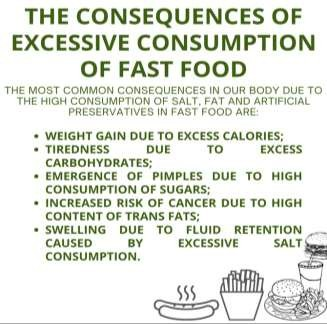
\includegraphics[width=\textwidth]{FIGURA01.jpg}
 \caption{Student post – exemplary of flyer.}
 \label{fig01}
 \source{Research corpus - Instagram: @change.yafood \cite[p.89]{oliveira2022}.}
\end{minipage}
\end{figure}

In the second exemplary, the poster, information about the risks of fast food consumption and about having a healthier diet is communicated to the interlocutors, as can be seen in \Cref{fig02}. 

\begin{figure}[h!]
\centering
\begin{minipage}{.99\textwidth}
 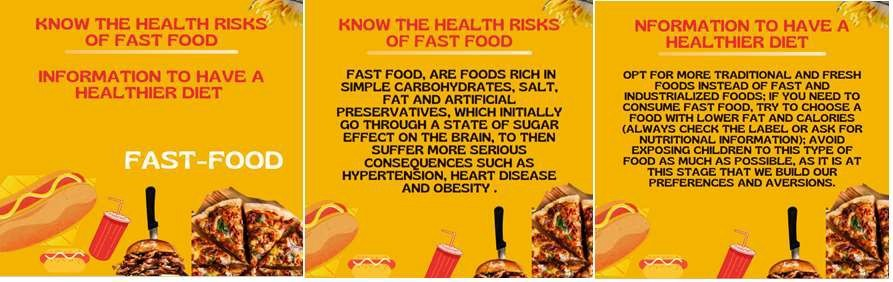
\includegraphics[width=\textwidth]{FIGURA2.jpg}
 \caption{Student post – sample poster.}
 \label{fig02}
 \source{Research corpus - Instagram: @change.yafood \cite[p.90]{oliveira2022}.}
\end{minipage}
\end{figure}

In this case, the verbal-visual text is organized in a carousel post on the platform, that is, a possibility of the Instagram social network itself, when upon publishing its text, the Instagram user selects more than 1 photo to post, creating links between them and producing a whole of meaning, which means that, in reception conditions, the interlocutors need to swipe the photo to the left to access the subsequent photo and the whole of the meaning of the post. The post had 3 photos that are part of the poster as a whole, one of which is the cover photo, in which the titles of the other 2 photos are present, repeated in them: \emph{Know the health risks of fast food, Information to have a healthier diet}. The first photo, therefore, consists of the 2 titles, while the second presents a definition of fast food (\emph{Fast food, are more foods rich in simple carbohydrates} [...]), characterized from the consequent risks of its consumption (hypertension, heart disease and obesity), and the third recommends the consumption alternatives (\emph{opt for more traditional and fresh […] try to choose [...]}). In addition, the hot dog, hamburger, soda and pizza images complement the intended meanings. In this case, the visual text not only illustrates the verbal text, but expands its meaning, bringing boundaries to what can be understood as foods that are rich in simple carbohydrates, salt, fat and artificial preservatives, informed through the verbal text in English language in the poster. In the following section, results are discussed.






\section{Discussion}
By integrating the analysis of the forms and types of discursive interaction, the forms of utterances and the forms of language in their usual linguistic conception, it is verified that the emergence of the students’ discourse in favor of healthy eating, starting from the context of teaching English inspired by the HCP, is the result of the predominance of the interrelation of this discourse with the discourse on the consequences of fast food in the lives of those who eat it. Thus, from a negative evaluative emphasis on fast food consumption manifested through bad consequences for the body and health of those who eat it - hypertension, heart disease, obesity and cancer (observed in \Cref{fig01} and \Cref{fig02}) - and, in addition, through the appeal for the consumption of alternative products - fresh food, checking the label (observed especially in \Cref{fig02}), the students’ utterances are addressed to the interlocutors in order to make them aware and try to promote a change in the daily social practice of these subjects.

At the same time, in the utterances, the use of expressions from the field of scientific activity is observed (\emph{trans fat, artificial preservatives, simple carbohydrate}), which points to the presence of technical discourse in the students’ posts, indicating that they mobilize the specialized contents that relate to their technical course in Nutrition and Dietetics: macro, micronutrients, etc., that is, concepts conceived within the scope of specialized scientific knowledge. Perceiving the presence of the discourse in favor of healthy eating and the technical discourse in the verbal-visual utterance produced by the students corroborates the assumption of the dialogic constitution of the utterances \cite{bakhtin_os_2016}.

Finally, it is worth highlighting, once again, that the visual text not only illustrates the verbal text but complements its meaning, evidencing a type of dialogical relationship of complementarity between these 2 languages, as predicted and verified in previous studies dedicated to the reading of verbal-visual utterances in the light of Dialogic Discourse Analysis \cite{brait_olhar_2013, limade2022auto}. The visual text presents examples of foods that should be avoided, pointing to the interrelationship between the discourse in favor of a healthy eating with that of everyday discourse, which points to possible foods consumed on a daily basis by people who may not be aware of the effects of this consumption: hot dogs, French fries, hamburgers, pizza, soda. It is also worth mentioning that, in this everyday discourse, when translating the non-verbal text into the verbal one, the impact of the English language is also observed from the expressions that are not translated in the Brazilian context: hot dog, hamburger and pizza.

Considering all this, when observing the dissemination of these discourses in a wide-ranging social network, it is possible to state that students both broaden their interlocutors beyond the more immediate context of the English language class (teachers and classmates) and commit to contribute to a society that is more aware of its eating habits, showing that the relationship between HCP and the teaching of English can contribute to increase the body of knowledge that reflects critical teaching of English, as perceived in previous research \cite[among others]{urzeda-freitas_educando_2012, costados2011visualizaccao, caetano_but_2020, mulico_learning_2020}. Next, some considerations are presented on the pedagogical and methodological implications of the research carried out.

\section{Final considerations}

In this article, the discourse of high school students in favor of healthy eating in the context of teaching English in a public school of professional education was analyzed, resulting in the elucidation of the constitution of this discourse through its interrelationship with the technical discourse, everyday discourse and discourse about the consequences of fast food consumption.

Thus, with regard to the pedagogical implications of the investigation, it is possible to conclude that, in the investigated context, student-participants in an action research with classes inspired by Historical-Critical Pedagogy demonstrated that they responded actively to proposals for reflection on the consumption of fast food, placing a negative value emphasis on this consumption, and, through the production of verbal-visual texts, exemplary of the flyer and the poster, they denounced the dangers of unhealthy food choices, in addition to making their interlocutors aware of this consumption, using a social network of great reach, Instagram.

With regard to the methodological implications of the investigation, the articulation between Dialogic Discourse Analysis and Historical-Critical Pedagogy is positively evaluated in order to propose an action research in the context of English language teaching at school. These theoretical-methodological choices proved to be capable of registering a relevant moment in the practice of research in language teaching, that is, the concrete response that the student-participants give to this process, from which it is possible to produce interpretations that collaborate with the evaluation of the process, promoting new concerns and proposals.

Articulating the dialogic perspective of language with other pedagogies explicitly committed to criticality, also guiding other social problems that are present in the daily lives of participants in the language teaching process - the difficulty in exercising citizenship, hate speech, among others - can constitute a challenge for new actions research interested in creating intelligibility about teaching and learning in other contexts, through the analysis of the discourses that are produced and circulate in them and beyond them.



\printbibliography\label{sec-bib}
% if the text is not in Portuguese, it might be necessary to use the code below instead to print the correct ABNT abbreviations [s.n.], [s.l.]
%\begin{portuguese}
%\printbibliography[title={Bibliography}]
%\end{portuguese}


%full list: conceptualization,datacuration,formalanalysis,funding,investigation,methodology,projadm,resources,software,supervision,validation,visualization,writing,review
\begin{contributors}[sec-contributors]
\authorcontribution{Elaine Cristina Gomes Aires de Oliveira}[conceptualization,datacuration,formalanalysis,methodology,validation,visualization,writing,review]
\authorcontribution{Samuel de Carvalho Lima}[conceptualization,datacuration,formalanalysis,methodology,validation,visualization,writing,review]
\end{contributors}



\end{document}

